\documentclass[aspectratio=169,12pt]{beamer}

\usepackage{tikz}
\usepackage{pgfplots}
\pgfplotsset{compat=1.18}
\usetikzlibrary{arrows.meta,positioning,shapes.geometric,fit,
                backgrounds,shadows,calc,decorations.pathmorphing}
\usepackage[T1]{fontenc}
\usepackage[utf8]{inputenc}
\usepackage{listings}
\usepackage{xcolor}
\usepackage{amsmath}
\usepackage{booktabs}
\usepackage{array}
\usepackage{graphicx}

%% ─────────────── COLOURS ───────────────
\definecolor{IceBlue}     {HTML}{E8F4FD}
\definecolor{SkyBlue}     {HTML}{AED6F1}
\definecolor{AccentBlue}  {HTML}{2980B9}
\definecolor{DeepBlue}    {HTML}{1A5276}
\definecolor{MintGreen}   {HTML}{D5F5E3}
\definecolor{AccentGreen} {HTML}{27AE60}
\definecolor{PeachOrange} {HTML}{FDEBD0}
\definecolor{AccentOrange}{HTML}{E67E22}
\definecolor{LavBlue}     {HTML}{EBF5FB}
\definecolor{SlateGray}   {HTML}{5D6D7E}
\definecolor{LightGray}   {HTML}{F2F3F4}
\definecolor{PurpleLight} {HTML}{E8DAEF}
\definecolor{AccentPurple}{HTML}{8E44AD}
\definecolor{YellowLight} {HTML}{FEF9E7}
\definecolor{AccentYellow}{HTML}{D4AC0D}
\definecolor{BgPage}      {HTML}{FAFBFC}

%% ─────────────── THEME ───────────────
\usetheme{default}
\setbeamertemplate{navigation symbols}{}
\setbeamercolor{background canvas}{bg=BgPage}
\setbeamercolor{frametitle}{fg=DeepBlue,bg=IceBlue}
\setbeamerfont{frametitle}{series=\bfseries,size=\large}

\setbeamertemplate{frametitle}{%
  \begin{tikzpicture}[overlay,remember picture]
    \fill[IceBlue] (current page.north west)
      rectangle ([yshift=-1.1cm]current page.north east);
    \draw[AccentBlue,line width=2pt]
      ([yshift=-1.1cm]current page.north west)
      -- ([yshift=-1.1cm]current page.north east);
  \end{tikzpicture}%
  \vspace{4pt}\hspace{8pt}\insertframetitle%
}

\setbeamertemplate{footline}{%
  \begin{tikzpicture}[overlay,remember picture]
    \fill[IceBlue] (current page.south west)
      rectangle ([yshift=0.55cm]current page.south east);
    \draw[AccentBlue,line width=1pt]
      ([yshift=0.55cm]current page.south west)
      -- ([yshift=0.55cm]current page.south east);
    \node[anchor=west,font=\tiny\color{SlateGray}]
      at ([xshift=8pt,yshift=0.27cm]current page.south west)
      {DistilBERT QA Pipeline --- Industrial Overview};
    \node[anchor=east,font=\tiny\color{SlateGray}]
      at ([xshift=-8pt,yshift=0.27cm]current page.south east)
      {\insertframenumber~/~\inserttotalframenumber};
  \end{tikzpicture}%
}

\setbeamercolor{itemize item}{fg=AccentBlue}
\setbeamertemplate{itemize item}{\small$\blacksquare$}
\setbeamercolor{block title}{fg=white,bg=AccentBlue}
\setbeamercolor{block body}{bg=IceBlue}

%% ─────────────── LISTING ───────────────
\lstdefinestyle{py}{
  language=Python,
  basicstyle=\ttfamily\scriptsize\color{DeepBlue},
  keywordstyle=\bfseries\color{AccentBlue},
  commentstyle=\itshape\color{SlateGray},
  stringstyle=\color{AccentGreen},
  numberstyle=\tiny\color{SlateGray},
  numbers=left, numbersep=6pt,
  backgroundcolor=\color{LavBlue},
  frame=single, framerule=0.5pt,
  rulecolor=\color{SkyBlue},
  breaklines=true, tabsize=4,
  showstringspaces=false,
  xleftmargin=10pt, xrightmargin=4pt,
}

%% ─────────────── TIKZ STYLES ───────────────
\tikzset{
  rbox/.style={rectangle,rounded corners=5pt,draw=#1!55,fill=#1!12,
               font=\small,minimum height=0.72cm,minimum width=5cm,
               text width=4.8cm,align=center},
  sbox/.style={rectangle,rounded corners=3pt,draw=SlateGray!40,
               fill=LightGray,font=\scriptsize\color{SlateGray}},
  tok/.style={rectangle,rounded corners=2pt,draw=#1!50,fill=#1!15,
              minimum width=1.05cm,minimum height=0.5cm,
              font=\fontsize{6.5}{7}\selectfont\bfseries\color{#1!70!black}},
  arr/.style={-Stealth,thick,color=SlateGray},
  barr/.style={-Stealth,very thick,color=AccentBlue},
}

%%==============================================
\begin{document}
%%==============================================

%% ─────────────── TITLE ───────────────
{
\setbeamertemplate{footline}{}
\begin{frame}[plain]
\begin{tikzpicture}[remember picture,overlay]

  \fill[IceBlue](current page.north west) rectangle (current page.south east);
  \fill[SkyBlue!30](current page.north west)
    rectangle ([yshift=-4.0cm]current page.north east);
  \fill[AccentBlue](current page.north west)
    rectangle ([yshift=-0.38cm]current page.north east);
  \draw[AccentBlue,line width=2pt]
    ([yshift=-4.0cm]current page.north west)
    -- ([yshift=-4.0cm]current page.north east);

  \node[text width=13cm,align=center]
    at ([yshift=-2.0cm]current page.north){
      {\fontsize{21}{25}\selectfont\bfseries\color{DeepBlue}
        DistilBERT Question-Answering Pipeline}\\[5pt]
      {\large\color{SlateGray} A Deep-Dive Industrial Overview}
    };

  \fill[AccentBlue!12]
    ([yshift=-4.4cm]current page.north west)
    rectangle ([yshift=-5.3cm]current page.north east);
  \node[font=\small\color{AccentBlue!80!black}]
    at ([yshift=-4.85cm]current page.north){
      \texttt{distilbert-base-cased-distilled-squad}
      \quad|\quad Extractive QA \quad|\quad HuggingFace Transformers
    };

  \node[rectangle,rounded corners=5pt,fill=AccentBlue!15,draw=AccentBlue!45,
        line width=1pt,minimum width=3.4cm,minimum height=1.1cm,
        text width=3.2cm,align=center,font=\scriptsize]
    at ([xshift=-5.5cm,yshift=-7.1cm]current page.north)
    {{\bfseries\color{DeepBlue}Architecture}\\[2pt]
     {\normalsize\bfseries\color{AccentBlue}DistilBERT 6L}};

  \node[rectangle,rounded corners=5pt,fill=AccentGreen!15,draw=AccentGreen!45,
        line width=1pt,minimum width=3.4cm,minimum height=1.1cm,
        text width=3.2cm,align=center,font=\scriptsize]
    at ([xshift=-1.8cm,yshift=-7.1cm]current page.north)
    {{\bfseries\color{DeepBlue}Parameters}\\[2pt]
     {\normalsize\bfseries\color{AccentGreen}66 Million}};

  \node[rectangle,rounded corners=5pt,fill=AccentOrange!15,draw=AccentOrange!45,
        line width=1pt,minimum width=3.4cm,minimum height=1.1cm,
        text width=3.2cm,align=center,font=\scriptsize]
    at ([xshift=1.8cm,yshift=-7.1cm]current page.north)
    {{\bfseries\color{DeepBlue}Fine-tuned on}\\[2pt]
     {\normalsize\bfseries\color{AccentOrange}SQuAD v1.1}};

  \node[rectangle,rounded corners=5pt,fill=AccentPurple!15,draw=AccentPurple!45,
        line width=1pt,minimum width=3.4cm,minimum height=1.1cm,
        text width=3.2cm,align=center,font=\scriptsize]
    at ([xshift=5.4cm,yshift=-7.1cm]current page.north)
    {{\bfseries\color{DeepBlue}Output}\\[2pt]
     {\normalsize\bfseries\color{AccentPurple}Answer + Score}};

  \fill[AccentBlue](current page.south west)
    rectangle ([yshift=0.38cm]current page.south east);
  \node[font=\tiny\color{white}]
    at ([yshift=0.19cm]current page.south)
    {Industrial Presentation \quad\textbullet\quad Built with \LaTeX{} Beamer + Ti\textit{k}Z};

\end{tikzpicture}
\end{frame}
}

%% ─────────────── SLIDE 2: AGENDA ───────────────
\begin{frame}{Agenda}
\vspace{0.15cm}
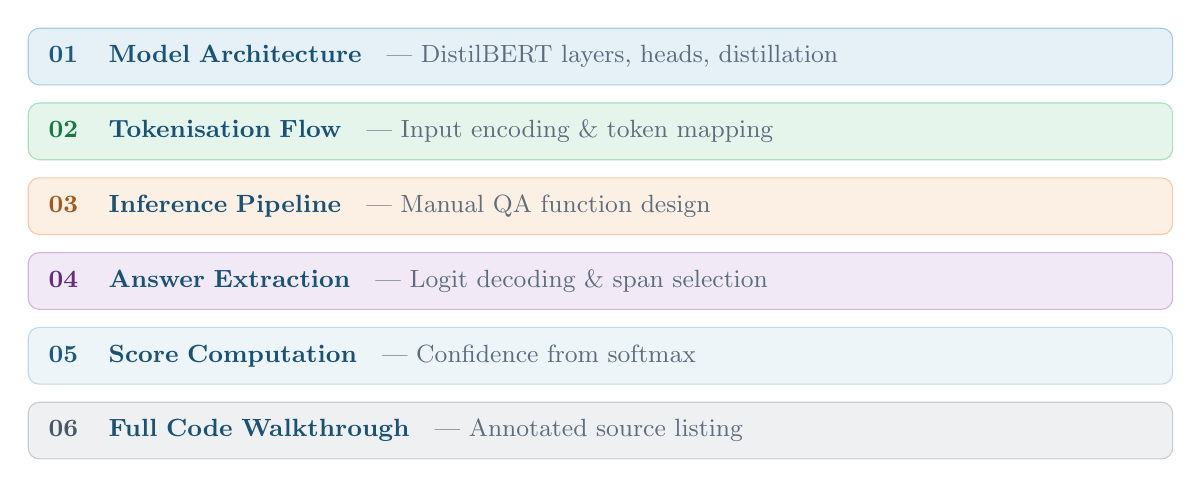
\begin{tikzpicture}

  \node[rectangle,rounded corners=4pt,fill=AccentBlue!12,draw=AccentBlue!40,
        minimum width=14.5cm,minimum height=0.72cm,text width=14.3cm,font=\small]
    at (0,0)
    {\hspace{4pt}\textcolor{AccentBlue!70!black}{\bfseries 01}\hspace{8pt}
     \textcolor{DeepBlue}{\bfseries Model Architecture}\hspace{6pt}
     \textcolor{SlateGray}{--- DistilBERT layers, heads, distillation}};

  \node[rectangle,rounded corners=4pt,fill=AccentGreen!12,draw=AccentGreen!40,
        minimum width=14.5cm,minimum height=0.72cm,text width=14.3cm,font=\small]
    at (0,-0.95)
    {\hspace{4pt}\textcolor{AccentGreen!70!black}{\bfseries 02}\hspace{8pt}
     \textcolor{DeepBlue}{\bfseries Tokenisation Flow}\hspace{6pt}
     \textcolor{SlateGray}{--- Input encoding \& token mapping}};

  \node[rectangle,rounded corners=4pt,fill=AccentOrange!12,draw=AccentOrange!40,
        minimum width=14.5cm,minimum height=0.72cm,text width=14.3cm,font=\small]
    at (0,-1.9)
    {\hspace{4pt}\textcolor{AccentOrange!70!black}{\bfseries 03}\hspace{8pt}
     \textcolor{DeepBlue}{\bfseries Inference Pipeline}\hspace{6pt}
     \textcolor{SlateGray}{--- Manual QA function design}};

  \node[rectangle,rounded corners=4pt,fill=AccentPurple!12,draw=AccentPurple!40,
        minimum width=14.5cm,minimum height=0.72cm,text width=14.3cm,font=\small]
    at (0,-2.85)
    {\hspace{4pt}\textcolor{AccentPurple!70!black}{\bfseries 04}\hspace{8pt}
     \textcolor{DeepBlue}{\bfseries Answer Extraction}\hspace{6pt}
     \textcolor{SlateGray}{--- Logit decoding \& span selection}};

  \node[rectangle,rounded corners=4pt,fill=AccentBlue!8,draw=AccentBlue!30,
        minimum width=14.5cm,minimum height=0.72cm,text width=14.3cm,font=\small]
    at (0,-3.8)
    {\hspace{4pt}\textcolor{AccentBlue!70!black}{\bfseries 05}\hspace{8pt}
     \textcolor{DeepBlue}{\bfseries Score Computation}\hspace{6pt}
     \textcolor{SlateGray}{--- Confidence from softmax}};

  \node[rectangle,rounded corners=4pt,fill=SlateGray!10,draw=SlateGray!35,
        minimum width=14.5cm,minimum height=0.72cm,text width=14.3cm,font=\small]
    at (0,-4.75)
    {\hspace{4pt}\textcolor{SlateGray!80!black}{\bfseries 06}\hspace{8pt}
     \textcolor{DeepBlue}{\bfseries Full Code Walkthrough}\hspace{6pt}
     \textcolor{SlateGray}{--- Annotated source listing}};

\end{tikzpicture}
\end{frame}

%% ─────────────── SLIDE 3: ARCHITECTURE ───────────────
\begin{frame}{01 --- DistilBERT Architecture}
\vspace{-0.8cm}
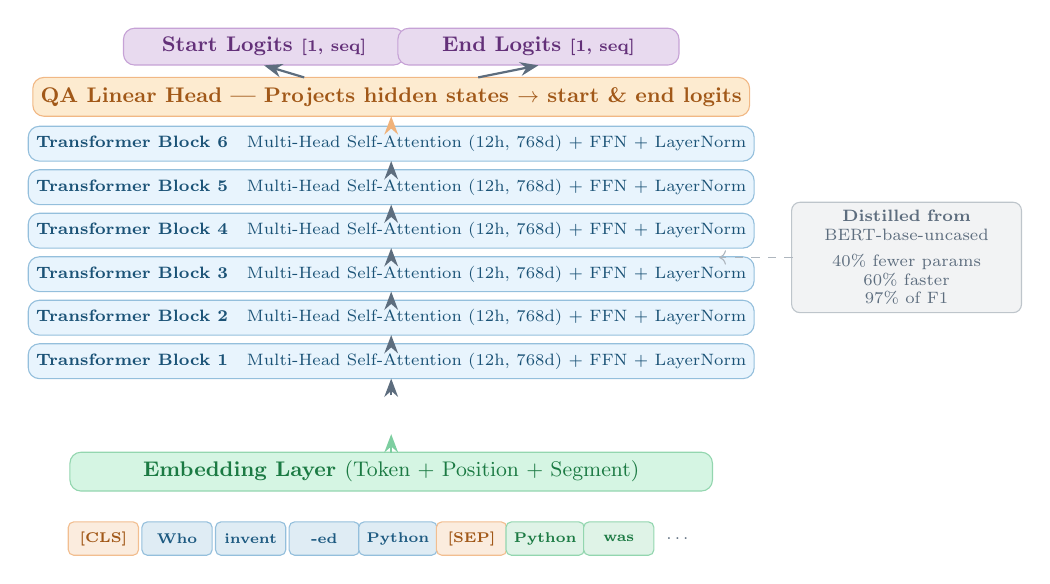
\begin{tikzpicture}[scale=0.85,transform shape]

  \node[tok=AccentOrange] at (0.0,-1)   {[CLS]};
  \node[tok=AccentBlue]   at (1.1,-1)   {Who};
  \node[tok=AccentBlue]   at (2.2,-1)   {invent};
  \node[tok=AccentBlue]   at (3.3,-1)   {-ed};
  \node[tok=AccentBlue]   at (4.4,-1)   {Python};
  \node[tok=AccentOrange] at (5.5,-1)   {[SEP]};
  \node[tok=AccentGreen]  at (6.6,-1)   {Python};
  \node[tok=AccentGreen]  at (7.7,-1)   {was};
  \node[font=\scriptsize\color{SlateGray}] at (8.6,-1) {\ldots};

  \node[rectangle,rounded corners=4pt,draw=AccentGreen!50,fill=MintGreen,
        minimum width=9.6cm,minimum height=0.58cm,
        font=\small\bfseries\color{AccentGreen!70!black}]
    at (4.3,0){Embedding Layer \small\normalfont(Token + Position + Segment)};
  \draw[arr,color=AccentGreen!60] (4.3,0.28) -- (4.3,0.56);

  \node[rectangle,rounded corners=4pt,draw=AccentBlue!50,fill=IceBlue,
        minimum width=9.6cm,minimum height=0.52cm,font=\scriptsize\color{DeepBlue}]
    at (4.3,1.65){\textbf{Transformer Block 1}\quad Multi-Head Self-Attention (12h, 768d) + FFN + LayerNorm};
  \node[rectangle,rounded corners=4pt,draw=AccentBlue!50,fill=IceBlue,
        minimum width=9.6cm,minimum height=0.52cm,font=\scriptsize\color{DeepBlue}]
    at (4.3,2.30){\textbf{Transformer Block 2}\quad Multi-Head Self-Attention (12h, 768d) + FFN + LayerNorm};
  \node[rectangle,rounded corners=4pt,draw=AccentBlue!50,fill=IceBlue,
        minimum width=9.6cm,minimum height=0.52cm,font=\scriptsize\color{DeepBlue}]
    at (4.3,2.95){\textbf{Transformer Block 3}\quad Multi-Head Self-Attention (12h, 768d) + FFN + LayerNorm};
  \node[rectangle,rounded corners=4pt,draw=AccentBlue!50,fill=IceBlue,
        minimum width=9.6cm,minimum height=0.52cm,font=\scriptsize\color{DeepBlue}]
    at (4.3,3.60){\textbf{Transformer Block 4}\quad Multi-Head Self-Attention (12h, 768d) + FFN + LayerNorm};
  \node[rectangle,rounded corners=4pt,draw=AccentBlue!50,fill=IceBlue,
        minimum width=9.6cm,minimum height=0.52cm,font=\scriptsize\color{DeepBlue}]
    at (4.3,4.25){\textbf{Transformer Block 5}\quad Multi-Head Self-Attention (12h, 768d) + FFN + LayerNorm};
  \node[rectangle,rounded corners=4pt,draw=AccentBlue!50,fill=IceBlue,
        minimum width=9.6cm,minimum height=0.52cm,font=\scriptsize\color{DeepBlue}]
    at (4.3,4.90){\textbf{Transformer Block 6}\quad Multi-Head Self-Attention (12h, 768d) + FFN + LayerNorm};

  \draw[arr] (4.3,1.14) -- (4.3,1.39);
  \draw[arr] (4.3,1.91) -- (4.3,2.04);
  \draw[arr] (4.3,2.56) -- (4.3,2.69);
  \draw[arr] (4.3,3.21) -- (4.3,3.34);
  \draw[arr] (4.3,3.86) -- (4.3,3.99);
  \draw[arr] (4.3,4.51) -- (4.3,4.64);

  \node[rectangle,rounded corners=4pt,draw=AccentOrange!55,fill=PeachOrange,
        minimum width=9.6cm,minimum height=0.58cm,
        font=\small\bfseries\color{AccentOrange!70!black}]
    at (4.3,5.60){QA Linear Head --- Projects hidden states $\rightarrow$ start \& end logits};
  \draw[arr,color=AccentOrange!60] (4.3,5.16) -- (4.3,5.31);

  \node[rectangle,rounded corners=4pt,draw=AccentPurple!50,fill=PurpleLight,
        minimum width=4.2cm,minimum height=0.55cm,
        font=\small\bfseries\color{AccentPurple!70!black}]
    at (2.4,6.35){Start Logits \scriptsize[1, seq]};
  \node[rectangle,rounded corners=4pt,draw=AccentPurple!50,fill=PurpleLight,
        minimum width=4.2cm,minimum height=0.55cm,
        font=\small\bfseries\color{AccentPurple!70!black}]
    at (6.5,6.35){End Logits \scriptsize[1, seq]};

  \draw[arr] (3.0,5.89) -- (2.4,6.07);
  \draw[arr] (5.6,5.89) -- (6.5,6.07);

  \node[sbox,text width=3.2cm,align=center]
    at (12.0,3.2)
    {\textbf{Distilled from}\\BERT-base-uncased\\[3pt]
     40\% fewer params\\60\% faster\\97\% of F1};
  \draw[dashed,SlateGray!50,->] (10.3,3.2) -- (9.2,3.2);

\end{tikzpicture}
\end{frame}

%% ─────────────── SLIDE 4: TOKENISATION ───────────────
\begin{frame}{02 --- Tokenisation Flow}
\vspace{0.2cm}
\begin{tikzpicture}[scale=0.9,transform shape]

  \node[rectangle,rounded corners=5pt,fill=LightGray,draw=SlateGray!40,
        minimum width=5.8cm,minimum height=0.65cm,font=\small\color{SlateGray}]
    (Q) at (0,5.6){Question: \textit{``Who invented Python?''}};
  \node[rectangle,rounded corners=5pt,fill=LightGray,draw=SlateGray!40,
        minimum width=6.2cm,minimum height=0.65cm,font=\small\color{SlateGray}]
    (C) at (8.5,5.6){Context: \textit{``Python was created by Guido\ldots''}};

  \node[rectangle,rounded corners=5pt,fill=MintGreen,draw=AccentGreen!50,
        minimum width=13.5cm,minimum height=0.65cm,
        font=\small\bfseries\color{AccentGreen!70!black}]
    (TOK) at (4.25,4.4){AutoTokenizer \small\normalfont(WordPiece, max\_length=512, truncation=True, return\_tensors=\textquotedbl pt\textquotedbl)};

  \draw[barr,color=AccentGreen!70] (Q.south)  -- ++(0,-0.35) -| ([xshift=-2cm]TOK.north);
  \draw[barr,color=AccentGreen!70] (C.south) -- ++(0,-0.35) -| ([xshift=2cm]TOK.north);

  \node[font=\scriptsize\color{SlateGray},anchor=west] at (-0.5,3.4){Token IDs:};
  \node[tok=AccentOrange] at (0.85,3.0){[CLS]};
  \node[tok=AccentBlue]   at (1.95,3.0){Who};
  \node[tok=AccentBlue]   at (3.05,3.0){in-};
  \node[tok=AccentBlue]   at (4.15,3.0){\#\#ven};
  \node[tok=AccentBlue]   at (5.25,3.0){\#\#ted};
  \node[tok=AccentBlue]   at (6.35,3.0){Python};
  \node[tok=AccentBlue]   at (7.45,3.0){?};
  \node[tok=AccentOrange] at (8.55,3.0){[SEP]};
  \node[tok=AccentGreen]  at (9.65,3.0){Python};
  \node[tok=AccentGreen]  at (10.75,3.0){was};
  \node[tok=AccentGreen]  at (11.85,3.0){\ldots};

  \node[font=\scriptsize\color{SlateGray},anchor=west] at (-0.5,2.35){Segment:};
  \node[rectangle,minimum width=1.05cm,minimum height=0.32cm,
        fill=AccentOrange!10,draw=AccentOrange!30,
        font=\fontsize{6}{7}\selectfont\color{AccentOrange!70!black}] at (0.85,2.1){A};
  \node[rectangle,minimum width=1.05cm,minimum height=0.32cm,
        fill=AccentBlue!10,draw=AccentBlue!30,
        font=\fontsize{6}{7}\selectfont\color{AccentBlue!70!black}] at (1.95,2.1){A};
  \node[rectangle,minimum width=1.05cm,minimum height=0.32cm,
        fill=AccentBlue!10,draw=AccentBlue!30,
        font=\fontsize{6}{7}\selectfont\color{AccentBlue!70!black}] at (3.05,2.1){A};
  \node[rectangle,minimum width=1.05cm,minimum height=0.32cm,
        fill=AccentBlue!10,draw=AccentBlue!30,
        font=\fontsize{6}{7}\selectfont\color{AccentBlue!70!black}] at (4.15,2.1){A};
  \node[rectangle,minimum width=1.05cm,minimum height=0.32cm,
        fill=AccentBlue!10,draw=AccentBlue!30,
        font=\fontsize{6}{7}\selectfont\color{AccentBlue!70!black}] at (5.25,2.1){A};
  \node[rectangle,minimum width=1.05cm,minimum height=0.32cm,
        fill=AccentBlue!10,draw=AccentBlue!30,
        font=\fontsize{6}{7}\selectfont\color{AccentBlue!70!black}] at (6.35,2.1){A};
  \node[rectangle,minimum width=1.05cm,minimum height=0.32cm,
        fill=AccentBlue!10,draw=AccentBlue!30,
        font=\fontsize{6}{7}\selectfont\color{AccentBlue!70!black}] at (7.45,2.1){A};
  \node[rectangle,minimum width=1.05cm,minimum height=0.32cm,
        fill=AccentOrange!10,draw=AccentOrange!30,
        font=\fontsize{6}{7}\selectfont\color{AccentOrange!70!black}] at (8.55,2.1){A};
  \node[rectangle,minimum width=1.05cm,minimum height=0.32cm,
        fill=AccentGreen!10,draw=AccentGreen!30,
        font=\fontsize{6}{7}\selectfont\color{AccentGreen!70!black}] at (9.65,2.1){B};
  \node[rectangle,minimum width=1.05cm,minimum height=0.32cm,
        fill=AccentGreen!10,draw=AccentGreen!30,
        font=\fontsize{6}{7}\selectfont\color{AccentGreen!70!black}] at (10.75,2.1){B};
  \node[rectangle,minimum width=1.05cm,minimum height=0.32cm,
        fill=AccentGreen!10,draw=AccentGreen!30,
        font=\fontsize{6}{7}\selectfont\color{AccentGreen!70!black}] at (11.85,2.1){B};

  \node[font=\scriptsize\color{SlateGray},anchor=west] at (-0.5,1.6)
    {\textbf{A} = Question tokens\quad \textbf{B} = Context tokens\quad
     \textcolor{AccentOrange!70!black}{\textbf{[CLS]/[SEP]}} = Special tokens};

  \node[rectangle,rounded corners=4pt,fill=IceBlue,draw=AccentBlue!40,
        minimum width=4.0cm,minimum height=0.6cm,
        font=\small\bfseries\color{DeepBlue}]
    (IID) at (1.5,0.5){input\_ids \scriptsize[1,L]};
  \node[rectangle,rounded corners=4pt,fill=IceBlue,draw=AccentBlue!40,
        minimum width=4.4cm,minimum height=0.6cm,
        font=\small\bfseries\color{DeepBlue}]
    (ATT) at (6.5,0.5){attention\_mask \scriptsize[1,L]};
  \node[rectangle,rounded corners=4pt,fill=IceBlue,draw=AccentBlue!40,
        minimum width=4.4cm,minimum height=0.6cm,
        font=\small\bfseries\color{DeepBlue}]
    (TID) at (11.5,0.5){token\_type\_ids \scriptsize[1,L]};

  \draw[barr,color=AccentBlue!60] (TOK.south west) ++(0.8,0) -- ++(0,-2.6) -- (IID.north);
  \draw[barr,color=AccentBlue!60] (TOK.south) -- (ATT.north);
  \draw[barr,color=AccentBlue!60] (TOK.south east) ++(-0.8,0) -- ++(0,-2.6) -- (TID.north);

\end{tikzpicture}
\end{frame}

%% ─────────────── SLIDE 5: PIPELINE ───────────────
\begin{frame}{03 --- Inference Pipeline Design}
\vspace{0.1cm}
\begin{center}
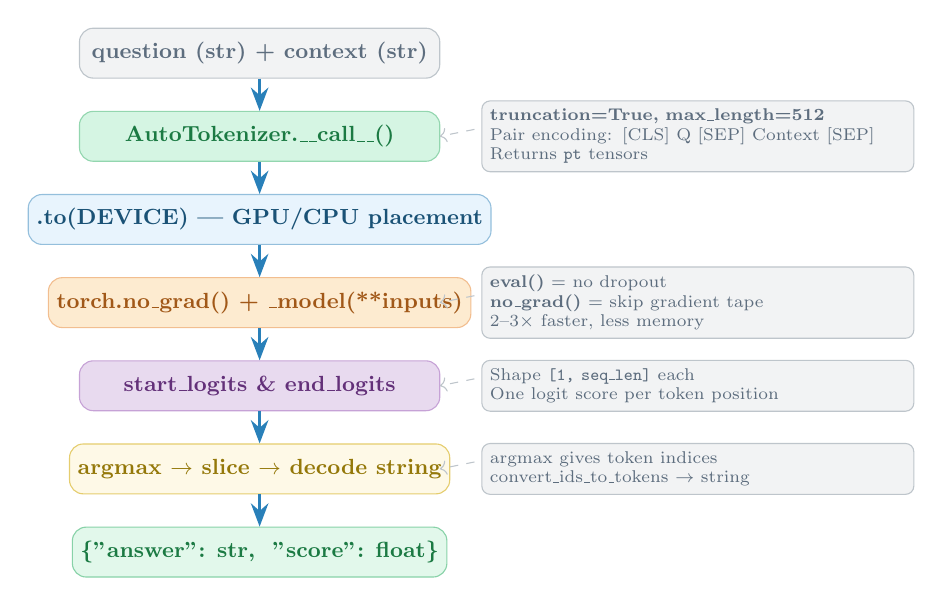
\begin{tikzpicture}[node distance=0.7cm,scale=0.88,transform shape]

  \node[rectangle,rounded corners=5pt,fill=LightGray,draw=SlateGray!40,
        minimum width=5.2cm,minimum height=0.72cm,font=\small\bfseries\color{SlateGray}]
    (IN) at (0,7.0){question (str) + context (str)};

  \node[rectangle,rounded corners=5pt,fill=MintGreen,draw=AccentGreen!50,
        minimum width=5.2cm,minimum height=0.72cm,
        font=\small\bfseries\color{AccentGreen!70!black}]
    (TOKN) at (0,5.8){AutoTokenizer.\_\_call\_\_()};

  \node[rectangle,rounded corners=5pt,fill=IceBlue,draw=AccentBlue!50,
        minimum width=5.2cm,minimum height=0.72cm,
        font=\small\bfseries\color{DeepBlue}]
    (DEV) at (0,4.6){.to(DEVICE) --- GPU/CPU placement};

  \node[rectangle,rounded corners=5pt,fill=PeachOrange,draw=AccentOrange!50,
        minimum width=5.2cm,minimum height=0.72cm,
        font=\small\bfseries\color{AccentOrange!70!black}]
    (FWD) at (0,3.4){torch.no\_grad() + \_model(**inputs)};

  \node[rectangle,rounded corners=5pt,fill=PurpleLight,draw=AccentPurple!50,
        minimum width=5.2cm,minimum height=0.72cm,
        font=\small\bfseries\color{AccentPurple!70!black}]
    (LOG) at (0,2.2){start\_logits \& end\_logits};

  \node[rectangle,rounded corners=5pt,fill=YellowLight,draw=AccentYellow!60,
        minimum width=5.2cm,minimum height=0.72cm,
        font=\small\bfseries\color{AccentYellow!70!black}]
    (SPAN) at (0,1.0){argmax $\to$ slice $\to$ decode string};

  \node[rectangle,rounded corners=5pt,fill=MintGreen!70,draw=AccentGreen!55,
        minimum width=5.2cm,minimum height=0.72cm,
        font=\small\bfseries\color{AccentGreen!70!black}]
    (OUT) at (0,-0.2){\{"answer": str,\ \ "score": float\}};

  \draw[barr] (IN.south)   -- (TOKN.north);
  \draw[barr] (TOKN.south) -- (DEV.north);
  \draw[barr] (DEV.south)  -- (FWD.north);
  \draw[barr] (FWD.south)  -- (LOG.north);
  \draw[barr] (LOG.south)  -- (SPAN.north);
  \draw[barr] (SPAN.south) -- (OUT.north);

  \node[sbox,text width=6.0cm,align=left,anchor=west] at (3.2,5.8)
    {\textbf{truncation=True, max\_length=512}\\
     Pair encoding: [CLS] Q [SEP] Context [SEP]\\
     Returns \texttt{pt} tensors};

  \node[sbox,text width=6.0cm,align=left,anchor=west] at (3.2,3.4)
    {\textbf{eval()} = no dropout\\
     \textbf{no\_grad()} = skip gradient tape\\
     2--3$\times$ faster, less memory};

  \node[sbox,text width=6.0cm,align=left,anchor=west] at (3.2,2.2)
    {Shape \texttt{[1, seq\_len]} each\\
     One logit score per token position};

  \node[sbox,text width=6.0cm,align=left,anchor=west] at (3.2,1.0)
    {argmax gives token indices\\
     convert\_ids\_to\_tokens $\to$ string};

  \draw[dashed,SlateGray!40,->] (3.1,5.9) -- (2.6,5.8);
  \draw[dashed,SlateGray!40,->] (3.1,3.5) -- (2.6,3.4);
  \draw[dashed,SlateGray!40,->] (3.1,2.3) -- (2.6,2.2);
  \draw[dashed,SlateGray!40,->] (3.1,1.1) -- (2.6,1.0);

\end{tikzpicture}
\end{center}
\end{frame}

%% ─────────────── SLIDE 6: SPAN EXTRACTION ───────────────
\begin{frame}{04 --- Answer Span Extraction}
\vspace{0.1cm}
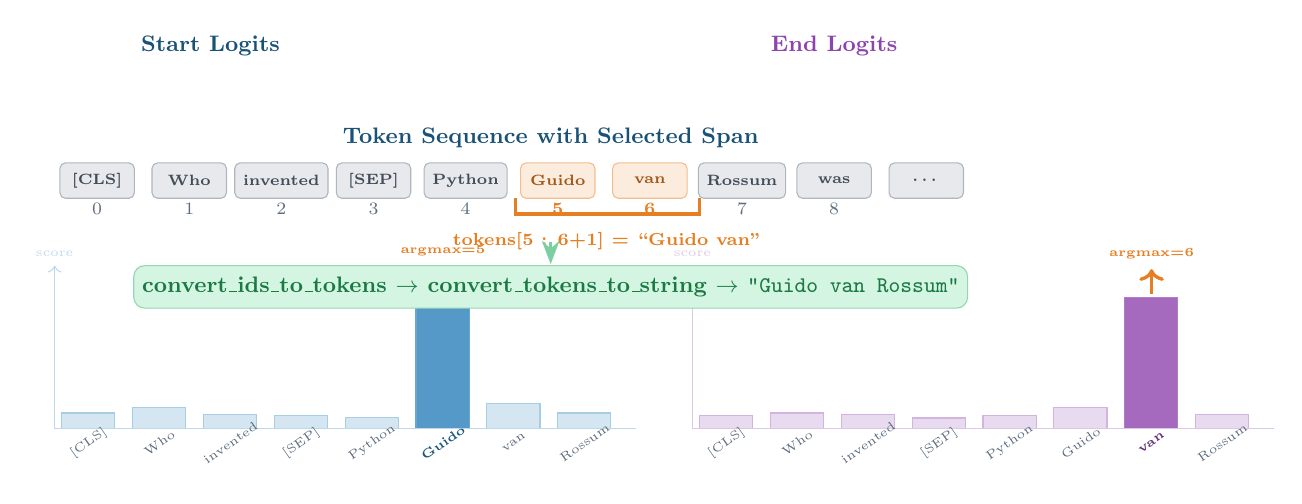
\begin{tikzpicture}[scale=0.9,transform shape]

  \node[font=\small\bfseries\color{DeepBlue}] at (2.2,5.6){Start Logits};
  \fill[AccentBlue!20] (0.1,0.2) rectangle (0.85,0.42);
  \fill[AccentBlue!20] (1.1,0.2) rectangle (1.85,0.50);
  \fill[AccentBlue!20] (2.1,0.2) rectangle (2.85,0.40);
  \fill[AccentBlue!20] (3.1,0.2) rectangle (3.85,0.38);
  \fill[AccentBlue!20] (4.1,0.2) rectangle (4.85,0.36);
  \fill[AccentBlue!80] (5.1,0.2) rectangle (5.85,2.10);
  \fill[AccentBlue!20] (6.1,0.2) rectangle (6.85,0.55);
  \fill[AccentBlue!20] (7.1,0.2) rectangle (7.85,0.42);

  \draw[AccentBlue!40] (0.1,0.2) rectangle (0.85,0.42);
  \draw[AccentBlue!40] (1.1,0.2) rectangle (1.85,0.50);
  \draw[AccentBlue!40] (2.1,0.2) rectangle (2.85,0.40);
  \draw[AccentBlue!40] (3.1,0.2) rectangle (3.85,0.38);
  \draw[AccentBlue!40] (4.1,0.2) rectangle (4.85,0.36);
  \draw[AccentBlue!70] (5.1,0.2) rectangle (5.85,2.10);
  \draw[AccentBlue!40] (6.1,0.2) rectangle (6.85,0.55);
  \draw[AccentBlue!40] (7.1,0.2) rectangle (7.85,0.42);

  \draw[AccentBlue!30,->] (0,0.2) -- (0,2.5) node[above,font=\tiny]{score};
  \draw[AccentBlue!30] (0,0.2) -- (8.2,0.2);

  \node[font=\fontsize{5.5}{6}\selectfont\color{SlateGray},rotate=35] at (0.48,0.0){[CLS]};
  \node[font=\fontsize{5.5}{6}\selectfont\color{SlateGray},rotate=35] at (1.48,0.0){Who};
  \node[font=\fontsize{5.5}{6}\selectfont\color{SlateGray},rotate=35] at (2.48,0.0){invented};
  \node[font=\fontsize{5.5}{6}\selectfont\color{SlateGray},rotate=35] at (3.48,0.0){[SEP]};
  \node[font=\fontsize{5.5}{6}\selectfont\color{SlateGray},rotate=35] at (4.48,0.0){Python};
  \node[font=\fontsize{5.5}{6}\selectfont\bfseries\color{AccentBlue!70!black},rotate=35] at (5.48,0.0){Guido};
  \node[font=\fontsize{5.5}{6}\selectfont\color{SlateGray},rotate=35] at (6.48,0.0){van};
  \node[font=\fontsize{5.5}{6}\selectfont\color{SlateGray},rotate=35] at (7.48,0.0){Rossum};

  \draw[->,AccentOrange,very thick] (5.48,2.15) -- ++(0,0.35)
    node[above,font=\tiny\bfseries\color{AccentOrange}]{argmax=5};

  \node[font=\small\bfseries\color{AccentPurple}] at (11.0,5.6){End Logits};
  \fill[AccentPurple!20] (9.1,0.2) rectangle (9.85,0.38);
  \fill[AccentPurple!20] (10.1,0.2) rectangle (10.85,0.42);
  \fill[AccentPurple!20] (11.1,0.2) rectangle (11.85,0.40);
  \fill[AccentPurple!20] (12.1,0.2) rectangle (12.85,0.35);
  \fill[AccentPurple!20] (13.1,0.2) rectangle (13.85,0.38);
  \fill[AccentPurple!20] (14.1,0.2) rectangle (14.85,0.50);
  \fill[AccentPurple!80] (15.1,0.2) rectangle (15.85,2.05);
  \fill[AccentPurple!20] (16.1,0.2) rectangle (16.85,0.40);

  \draw[AccentPurple!40] (9.1,0.2) rectangle (9.85,0.38);
  \draw[AccentPurple!40] (10.1,0.2) rectangle (10.85,0.42);
  \draw[AccentPurple!40] (11.1,0.2) rectangle (11.85,0.40);
  \draw[AccentPurple!40] (12.1,0.2) rectangle (12.85,0.35);
  \draw[AccentPurple!40] (13.1,0.2) rectangle (13.85,0.38);
  \draw[AccentPurple!40] (14.1,0.2) rectangle (14.85,0.50);
  \draw[AccentPurple!70] (15.1,0.2) rectangle (15.85,2.05);
  \draw[AccentPurple!40] (16.1,0.2) rectangle (16.85,0.40);

  \draw[AccentPurple!30,->] (9.0,0.2) -- (9.0,2.5) node[above,font=\tiny]{score};
  \draw[AccentPurple!30] (9.0,0.2) -- (17.2,0.2);

  \node[font=\fontsize{5.5}{6}\selectfont\color{SlateGray},rotate=35] at (9.48,0.0){[CLS]};
  \node[font=\fontsize{5.5}{6}\selectfont\color{SlateGray},rotate=35] at (10.48,0.0){Who};
  \node[font=\fontsize{5.5}{6}\selectfont\color{SlateGray},rotate=35] at (11.48,0.0){invented};
  \node[font=\fontsize{5.5}{6}\selectfont\color{SlateGray},rotate=35] at (12.48,0.0){[SEP]};
  \node[font=\fontsize{5.5}{6}\selectfont\color{SlateGray},rotate=35] at (13.48,0.0){Python};
  \node[font=\fontsize{5.5}{6}\selectfont\color{SlateGray},rotate=35] at (14.48,0.0){Guido};
  \node[font=\fontsize{5.5}{6}\selectfont\bfseries\color{AccentPurple!70!black},rotate=35] at (15.48,0.0){van};
  \node[font=\fontsize{5.5}{6}\selectfont\color{SlateGray},rotate=35] at (16.48,0.0){Rossum};

  \draw[->,AccentOrange,very thick] (15.48,2.10) -- ++(0,0.35)
    node[above,font=\tiny\bfseries\color{AccentOrange}]{argmax=6};

  \node[font=\small\bfseries\color{DeepBlue}] at (7.0,4.3){Token Sequence with Selected Span};
  \node[tok=SlateGray]    at (0.6,3.7){[CLS]};
  \node[tok=SlateGray]    at (1.9,3.7){Who};
  \node[tok=SlateGray]    at (3.2,3.7){invented};
  \node[tok=SlateGray]    at (4.5,3.7){[SEP]};
  \node[tok=SlateGray]    at (5.8,3.7){Python};
  \node[tok=AccentOrange] at (7.1,3.7){\textbf{Guido}};
  \node[tok=AccentOrange] at (8.4,3.7){\textbf{van}};
  \node[tok=SlateGray]    at (9.7,3.7){Rossum};
  \node[tok=SlateGray]    at (11.0,3.7){was};
  \node[tok=SlateGray]    at (12.3,3.7){\ldots};

  \node[font=\scriptsize\color{SlateGray}]   at (0.6,3.3){0};
  \node[font=\scriptsize\color{SlateGray}]   at (1.9,3.3){1};
  \node[font=\scriptsize\color{SlateGray}]   at (3.2,3.3){2};
  \node[font=\scriptsize\color{SlateGray}]   at (4.5,3.3){3};
  \node[font=\scriptsize\color{SlateGray}]   at (5.8,3.3){4};
  \node[font=\scriptsize\bfseries\color{AccentOrange}] at (7.1,3.3){5};
  \node[font=\scriptsize\bfseries\color{AccentOrange}] at (8.4,3.3){6};
  \node[font=\scriptsize\color{SlateGray}]   at (9.7,3.3){7};
  \node[font=\scriptsize\color{SlateGray}]   at (11.0,3.3){8};

  \draw[AccentOrange,very thick] (6.5,3.45) -- ++(0,-0.22) -- ++(2.6,0) -- ++(0,0.22);
  \node[font=\scriptsize\bfseries\color{AccentOrange}] at (7.8,2.85)
    {tokens[5 : 6+1] = ``Guido van''};

  \node[rectangle,rounded corners=4pt,fill=MintGreen,draw=AccentGreen!50,
        minimum width=10.5cm,minimum height=0.6cm,
        font=\small\bfseries\color{AccentGreen!70!black}]
    at (7.0,2.2){
      convert\_ids\_to\_tokens $\to$ convert\_tokens\_to\_string $\to$ \texttt{"Guido van Rossum"}
    };
  \draw[barr,color=AccentGreen!60] (7.0,2.83) -- (7.0,2.52);

\end{tikzpicture}
\end{frame}

%% ─────────────── SLIDE 7: SCORE ───────────────
\begin{frame}{05 --- Confidence Score Computation}
\vspace{0.2cm}
\begin{columns}[T]
\column{0.52\textwidth}

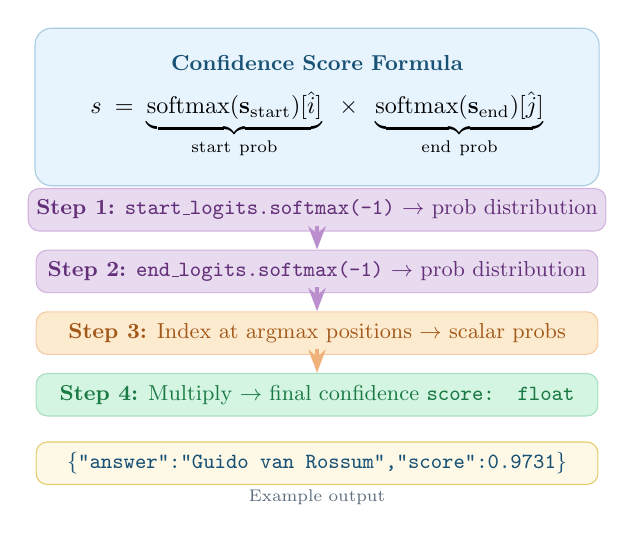
\begin{tikzpicture}[scale=0.87,transform shape]

  \node[rectangle,rounded corners=6pt,fill=IceBlue,draw=AccentBlue!40,
        minimum width=8.2cm,minimum height=2.3cm,text width=8.0cm,align=center]
    at (4.0,5.6){
      {\small\bfseries\color{DeepBlue}Confidence Score Formula}\\[6pt]
      $\displaystyle
        s = \underbrace{\mathrm{softmax}(\mathbf{s}_{\mathrm{start}})[\hat{i}]}_{\text{start prob}}
        \;\times\;
        \underbrace{\mathrm{softmax}(\mathbf{s}_{\mathrm{end}})[\hat{j}]}_{\text{end prob}}$
    };

  \node[rectangle,rounded corners=4pt,fill=PurpleLight,draw=AccentPurple!40,
        minimum width=8.2cm,minimum height=0.62cm,font=\small\color{AccentPurple!70!black}]
    at (4.0,4.1){\textbf{Step 1:}
      \texttt{start\_logits.softmax(-1)} $\to$ prob distribution};

  \node[rectangle,rounded corners=4pt,fill=PurpleLight,draw=AccentPurple!40,
        minimum width=8.2cm,minimum height=0.62cm,font=\small\color{AccentPurple!70!black}]
    at (4.0,3.2){\textbf{Step 2:}
      \texttt{end\_logits.softmax(-1)} $\to$ prob distribution};

  \node[rectangle,rounded corners=4pt,fill=PeachOrange,draw=AccentOrange!40,
        minimum width=8.2cm,minimum height=0.62cm,font=\small\color{AccentOrange!70!black}]
    at (4.0,2.3){\textbf{Step 3:} Index at argmax positions $\to$ scalar probs};

  \node[rectangle,rounded corners=4pt,fill=MintGreen,draw=AccentGreen!40,
        minimum width=8.2cm,minimum height=0.62cm,font=\small\color{AccentGreen!70!black}]
    at (4.0,1.4){\textbf{Step 4:} Multiply $\to$ final confidence \texttt{score: float}};

  \draw[barr,color=AccentPurple!60] (4.0,3.87) -- (4.0,3.52);
  \draw[barr,color=AccentPurple!60] (4.0,2.97) -- (4.0,2.62);
  \draw[barr,color=AccentOrange!60] (4.0,2.07) -- (4.0,1.72);

  \node[rectangle,rounded corners=4pt,fill=YellowLight,draw=AccentYellow!60,
        minimum width=8.2cm,minimum height=0.62cm,font=\ttfamily\small\color{DeepBlue}]
    at (4.0,0.4)%
    {\{"answer":"Guido van Rossum","score":0.9731\}};
  \node[font=\scriptsize\color{SlateGray}] at (4.0,-0.1){Example output};

\end{tikzpicture}

\column{0.45\textwidth}
\vspace{0.3cm}
{\small\bfseries\color{DeepBlue}Score Interpretation}\\[8pt]

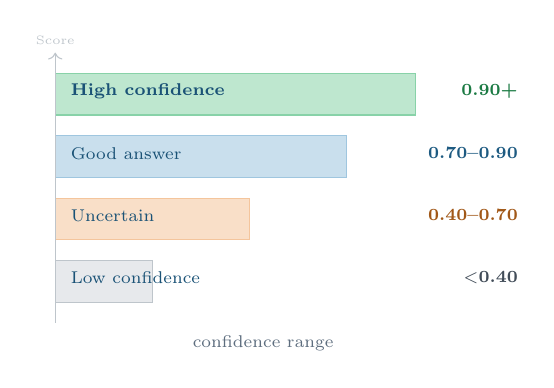
\begin{tikzpicture}[scale=0.88,transform shape]

  \fill[AccentGreen!30] (0,3.6) rectangle (5.2,4.2);
  \draw[AccentGreen!55] (0,3.6) rectangle (5.2,4.2);
  \node[anchor=west,font=\scriptsize\color{DeepBlue}] at (0.1,3.95){\textbf{High confidence}};
  \node[anchor=east,font=\scriptsize\bfseries\color{AccentGreen!70!black}] at (6.8,3.95){0.90+};

  \fill[AccentBlue!25] (0,2.7) rectangle (4.2,3.3);
  \draw[AccentBlue!45] (0,2.7) rectangle (4.2,3.3);
  \node[anchor=west,font=\scriptsize\color{DeepBlue}] at (0.1,3.05){Good answer};
  \node[anchor=east,font=\scriptsize\bfseries\color{AccentBlue!70!black}] at (6.8,3.05){0.70--0.90};

  \fill[AccentOrange!25] (0,1.8) rectangle (2.8,2.4);
  \draw[AccentOrange!45] (0,1.8) rectangle (2.8,2.4);
  \node[anchor=west,font=\scriptsize\color{DeepBlue}] at (0.1,2.15){Uncertain};
  \node[anchor=east,font=\scriptsize\bfseries\color{AccentOrange!70!black}] at (6.8,2.15){0.40--0.70};

  \fill[SlateGray!15] (0,0.9) rectangle (1.4,1.5);
  \draw[SlateGray!40] (0,0.9) rectangle (1.4,1.5);
  \node[anchor=west,font=\scriptsize\color{DeepBlue}] at (0.1,1.25){Low confidence};
  \node[anchor=east,font=\scriptsize\bfseries\color{SlateGray!70!black}] at (6.8,1.25){$<$0.40};

  \draw[SlateGray!40,->] (0,0.6) -- (0,4.5) node[above,font=\tiny]{Score};
  \node[font=\scriptsize\color{SlateGray}] at (3.0,0.3){confidence range};

\end{tikzpicture}

\vspace{0.4cm}
{\scriptsize\color{SlateGray}
Product of two independent softmaxes. True joint
scoring uses a 2-D score matrix, but this approach
is efficient and standard practice in extractive QA.}
\end{columns}
\end{frame}

%% ─────────────── SLIDE 8: CODE ───────────────
\begin{frame}[fragile]{06 --- Full Code Walkthrough}
\vspace{0.1cm}
\begin{columns}[T]
\column{0.55\textwidth}
\begin{lstlisting}[style=py,title={\texttt{distilbert\_qa.py}}]
from transformers import (
    AutoTokenizer,
    AutoModelForQuestionAnswering
)
import torch

MODEL = "distilbert-base-cased-distilled-squad"

# Load once -- reuse many times
_tok   = AutoTokenizer.from_pretrained(MODEL)
_model = AutoModelForQuestionAnswering\
           .from_pretrained(MODEL).to(DEVICE)
_model.eval()      # disable dropout

def qa_distilbert(question: str,
                  context: str) -> dict:
    # 1. Tokenise (PT tensors on device)
    inputs = _tok(question, context,
        return_tensors="pt",
        truncation=True,
        max_length=512).to(DEVICE)

    # 2. Forward pass (no gradient)
    with torch.no_grad():
        out = _model(**inputs)

    # 3. Decode answer span
    s = out.start_logits.argmax()
    e = out.end_logits.argmax() + 1
    ids    = inputs["input_ids"][0][s:e]
    tokens = _tok.convert_ids_to_tokens(ids)
    answer = _tok.convert_tokens_to_string(
                 tokens)

    # 4. Confidence score
    sp = out.start_logits.softmax(-1)[0][s]\
           .item()
    ep = out.end_logits.softmax(-1)[0][e-1]\
           .item()

    return {"answer": answer,
            "score":  sp * ep}
\end{lstlisting}

\column{0.42\textwidth}
\vspace{0.2cm}

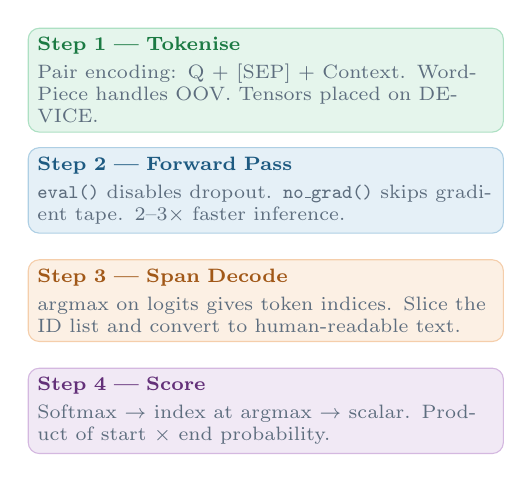
\begin{tikzpicture}

  \node[rectangle,rounded corners=4pt,fill=AccentGreen!12,draw=AccentGreen!38,
        minimum width=6.0cm,text width=5.8cm,
        minimum height=1.0cm,font=\scriptsize] at (0,0)
    {\textcolor{AccentGreen!70!black}{\bfseries Step 1 --- Tokenise}\\[2pt]
     \textcolor{SlateGray}{Pair encoding: Q + [SEP] + Context.
     WordPiece handles OOV. Tensors placed on DEVICE.}};

  \node[rectangle,rounded corners=4pt,fill=AccentBlue!12,draw=AccentBlue!38,
        minimum width=6.0cm,text width=5.8cm,
        minimum height=1.0cm,font=\scriptsize] at (0,-1.4)
    {\textcolor{AccentBlue!70!black}{\bfseries Step 2 --- Forward Pass}\\[2pt]
     \textcolor{SlateGray}{\texttt{eval()} disables dropout.
     \texttt{no\_grad()} skips gradient tape.
     2--3$\times$ faster inference.}};

  \node[rectangle,rounded corners=4pt,fill=AccentOrange!12,draw=AccentOrange!38,
        minimum width=6.0cm,text width=5.8cm,
        minimum height=1.0cm,font=\scriptsize] at (0,-2.8)
    {\textcolor{AccentOrange!70!black}{\bfseries Step 3 --- Span Decode}\\[2pt]
     \textcolor{SlateGray}{argmax on logits gives token indices.
     Slice the ID list and convert to human-readable text.}};

  \node[rectangle,rounded corners=4pt,fill=AccentPurple!12,draw=AccentPurple!38,
        minimum width=6.0cm,text width=5.8cm,
        minimum height=1.0cm,font=\scriptsize] at (0,-4.2)
    {\textcolor{AccentPurple!70!black}{\bfseries Step 4 --- Score}\\[2pt]
     \textcolor{SlateGray}{Softmax $\to$ index at argmax $\to$ scalar.
     Product of start $\times$ end probability.}};

\end{tikzpicture}

\end{columns}
\end{frame}

%% ─────────────── SLIDE 9: SUMMARY ───────────────
\begin{frame}{System Summary \& Key Design Choices}
\vspace{0.1cm}
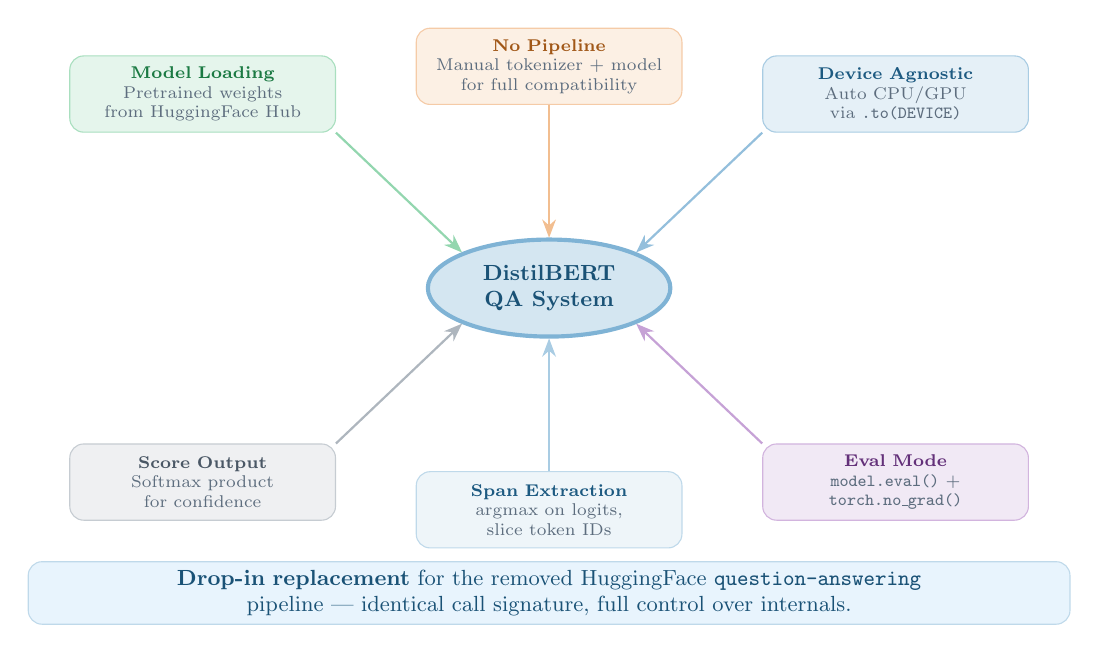
\begin{tikzpicture}[scale=0.88,transform shape]

  \node[ellipse,fill=AccentBlue!20,draw=AccentBlue!60,line width=1.5pt,
        minimum width=3.5cm,minimum height=1.4cm,
        font=\small\bfseries\color{DeepBlue},align=center]
    (C) at (7.0,3.0){DistilBERT\\QA System};

  \node[rectangle,rounded corners=5pt,fill=AccentGreen!12,draw=AccentGreen!40,
        minimum width=3.8cm,minimum height=1.1cm,text width=3.6cm,align=center,
        font=\scriptsize] (A) at (2.0,5.8)
    {\textcolor{AccentGreen!70!black}{\bfseries Model Loading}\\
     \textcolor{SlateGray}{Pretrained weights\\from HuggingFace Hub}};

  \node[rectangle,rounded corners=5pt,fill=AccentOrange!12,draw=AccentOrange!40,
        minimum width=3.8cm,minimum height=1.1cm,text width=3.6cm,align=center,
        font=\scriptsize] (B) at (7.0,6.2)
    {\textcolor{AccentOrange!70!black}{\bfseries No Pipeline}\\
     \textcolor{SlateGray}{Manual tokenizer + model\\for full compatibility}};

  \node[rectangle,rounded corners=5pt,fill=AccentBlue!12,draw=AccentBlue!40,
        minimum width=3.8cm,minimum height=1.1cm,text width=3.6cm,align=center,
        font=\scriptsize] (D) at (12.0,5.8)
    {\textcolor{AccentBlue!70!black}{\bfseries Device Agnostic}\\
     \textcolor{SlateGray}{Auto CPU/GPU\\via \texttt{.to(DEVICE)}}};

  \node[rectangle,rounded corners=5pt,fill=AccentPurple!12,draw=AccentPurple!40,
        minimum width=3.8cm,minimum height=1.1cm,text width=3.6cm,align=center,
        font=\scriptsize] (E) at (12.0,0.2)
    {\textcolor{AccentPurple!70!black}{\bfseries Eval Mode}\\
     \textcolor{SlateGray}{\texttt{model.eval()} +\\
     \texttt{torch.no\_grad()}}};

  \node[rectangle,rounded corners=5pt,fill=AccentBlue!8,draw=AccentBlue!30,
        minimum width=3.8cm,minimum height=1.1cm,text width=3.6cm,align=center,
        font=\scriptsize] (F) at (7.0,-0.2)
    {\textcolor{AccentBlue!70!black}{\bfseries Span Extraction}\\
     \textcolor{SlateGray}{argmax on logits,\\slice token IDs}};

  \node[rectangle,rounded corners=5pt,fill=SlateGray!10,draw=SlateGray!35,
        minimum width=3.8cm,minimum height=1.1cm,text width=3.6cm,align=center,
        font=\scriptsize] (G) at (2.0,0.2)
    {\textcolor{SlateGray!80!black}{\bfseries Score Output}\\
     \textcolor{SlateGray}{Softmax product\\for confidence}};

  \draw[thick,AccentGreen!50,-Stealth]  (A.south east) -- (C.north west);
  \draw[thick,AccentOrange!50,-Stealth] (B.south)      -- (C.north);
  \draw[thick,AccentBlue!50,-Stealth]   (D.south west) -- (C.north east);
  \draw[thick,AccentPurple!50,-Stealth] (E.north west) -- (C.south east);
  \draw[thick,AccentBlue!40,-Stealth]   (F.north)      -- (C.south);
  \draw[thick,SlateGray!50,-Stealth]    (G.north east) -- (C.south west);

  \node[rectangle,rounded corners=5pt,fill=IceBlue,draw=AccentBlue!30,
        minimum width=15.0cm,minimum height=0.72cm,text width=14.8cm,align=center,
        font=\small\color{DeepBlue}]
    at (7.0,-1.4)
    {\textbf{Drop-in replacement} for the removed HuggingFace
     \texttt{question-answering} pipeline ---
     identical call signature, full control over internals.};

\end{tikzpicture}
\end{frame}

%% ─────────────── THANK YOU ───────────────
{
\setbeamertemplate{footline}{}
\begin{frame}[plain]
\begin{tikzpicture}[remember picture,overlay]
  \fill[IceBlue](current page.north west) rectangle (current page.south east);
  \fill[AccentBlue](current page.north west)
    rectangle ([yshift=-0.4cm]current page.north east);
  \fill[AccentBlue](current page.south west)
    rectangle ([yshift=0.4cm]current page.south east);

  \node[font=\fontsize{26}{30}\selectfont\bfseries\color{DeepBlue},anchor=center]
    at ([yshift=1.5cm]current page.center){Thank You};

  \node[font=\normalsize\color{SlateGray},anchor=center]
    at ([yshift=0.5cm]current page.center)
    {DistilBERT QA Pipeline --- Industrial Deep Dive};

  \draw[AccentBlue!40,line width=1pt]
    ([xshift=-2.5cm,yshift=0.1cm]current page.center)
    -- ([xshift=2.5cm,yshift=0.1cm]current page.center);

  \node[rectangle,rounded corners=6pt,fill=AccentBlue!15,draw=AccentBlue!40,
        minimum width=3.2cm,minimum height=1.2cm,align=center,font=\small]
    at ([xshift=-4.5cm,yshift=-1.4cm]current page.center)
    {{\large\bfseries\color{AccentBlue}66M}\\[2pt]{\scriptsize\color{SlateGray}Parameters}};

  \node[rectangle,rounded corners=6pt,fill=AccentGreen!15,draw=AccentGreen!40,
        minimum width=3.2cm,minimum height=1.2cm,align=center,font=\small]
    at ([xshift=0cm,yshift=-1.4cm]current page.center)
    {{\large\bfseries\color{AccentGreen}6}\\[2pt]{\scriptsize\color{SlateGray}Transformer Layers}};

  \node[rectangle,rounded corners=6pt,fill=AccentOrange!15,draw=AccentOrange!40,
        minimum width=3.2cm,minimum height=1.2cm,align=center,font=\small]
    at ([xshift=4.5cm,yshift=-1.4cm]current page.center)
    {{\large\bfseries\color{AccentOrange}SQuAD}\\[2pt]{\scriptsize\color{SlateGray}Fine-tune Dataset}};
\end{tikzpicture}
\end{frame}
}

\end{document}